\documentclass{beamer}
\usetheme{Boadilla}
\usepackage{animate}
\usepackage{bibentry}


\title{Unmanned Aerial Vehicle Swarm Intelligence}
\subtitle{An exploration of pathfinding and control for UAV swarms using swarm algorithms.}
\author{Antonio Brito}
\institute{University of Warwick}
\date{\today}

\begin{document}


\begin{frame}
    \titlepage
\end{frame}

\section{Overview}

\begin{frame}
    \frametitle{Unmanned Aerial Vehicles}
    UAVs have a wide range of scientific applications:
    \begin{itemize}
        \item Area Reconnaissance \& Surveying
        \item Mapping \& Environmental Monitoring
        \item Agricultural
        \item Military
        \item Search \& Rescue
    \end{itemize}
    
    UAVs are cheap \& swarms introduce redundancy and the ability to work together.
\end{frame}

\begin{frame}
    \frametitle{UAV Swarms}
    UAVs have a wide range of scientific applications:
    \begin{itemize}
        \item Area Reconnaissance \& Surveying: Increased coverage and accuracy
        \item Mapping \& Environmental Monitoring: Faster
        \item Agricultural: Increased coverage and accuracy
        \item Military: Increased redundancy
        \item Search \& Rescue: Increased redundancy
    \end{itemize}
    
    UAVs are cheap \& swarms introduce redundancy and the ability to work together.
    \\
    Can we utilise emergent, natural behaviour as part of autonomy?
\end{frame}

\section{Methodology}
\subsection{Physics Modelling}

\begin{frame}
    \frametitle{Unity}
    \onslide<1->{We will use Unity, a game development platform, to model our UAV swarm and the surrounding environment.}
    \\
    \onslide<1->{Inspiration: \emph{Boids} by Sebastian Lague}
    \\
    \begin{figure}
        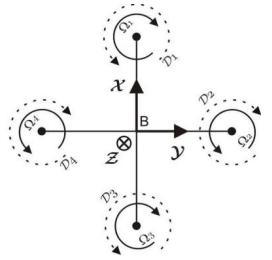
\includegraphics[scale=0.3]{prop}
        \caption{Quadcopter Model}\cite{Bouabdallah}
    \end{figure}
    \onslide<2->{Our first challenge is controlling the movement of the quadcopters.}
\end{frame}

\begin{frame}
    \frametitle{PID Control}
    \onslide<1->{
        We will use a PID controller to control the movement of the quadcopters.
        \\
        We can define a goal orientation and the PID controller will adjust the motors to achieve this orientation.
    }
    \bigskip
    \onslide<1->{
    \begin{columns}
        \column{0.33\textwidth}
        \centering
        \onslide<1->{Proportional}
        \onslide<1->{
        $$
        P = K_p e(t)
        $$
        }
        \column{0.33\textwidth}
        \centering
        \onslide<1->{Integral}
        \onslide<1->{
        $$
        I = K_i \int_0^t e(t) dt
        $$
        }
        \column{0.33\textwidth}
        \centering
        \onslide<1->{Derivative}
        \onslide<1->{
        $$
        D = K_d \frac{d}{dt} e(t)
        $$
        }
        \end{columns}
    }
\end{frame}

\subsection{Boids}
\begin{frame}
    \frametitle{Swarming Algorithm}
    \onslide<1->{1987: Craig Reynolds' Boids}
    \\
    \onslide<1->{Simulates the emergent behaviour present in flocks of birds.}
    \\
    \begin{itemize}
        \item Square Avoidance Radius $R_{av}^2$
        \item Neighbourhood $N$
        \item Agent Position $\vec{a}$
    \end{itemize}
\end{frame}


\begin{frame}
    \frametitle{Avoidance}
    \only<1>{
        \begin{figure}
            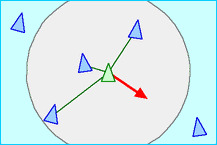
\includegraphics[scale=0.4]{se-0000}
            \caption{Avoidance Rule\cite{boids}}
        \end{figure}
    }
    \only<1>{The avoidance rule ensures that agents do not collide with each other.}
    \only<1>{This can be done by calculating the average position of the agents in the neighbourhood.}
    \only<1->{
    
    The avoidance move vector $\vec{A}$ can be represented as follows:
    
    \[
    \vec{A} = \begin{cases}
    0 & \text{if } |N| = 0 \\
    \frac{1}{n_{avoid}}\sum_{n=1}^{|N|} \vec{a} - \vec{n} , \vec{a} - \vec{n} < R_{av}^2  & \text{otherwise}
    \end{cases}
    \]
    
    with $n_{avoid}$, the number of neighbors for which the adjustment is non-zero.
    \\
    
    }

\end{frame}

\begin{frame}
    \frametitle{Alignment}
    \onslide<1->{
        \begin{figure}
            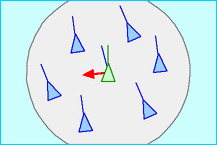
\includegraphics[scale=0.5]{al-0000}
            \caption{Alignment Rule\cite{boids}}
        \end{figure}
        The alignment rule ensures agents match the heading and velocity of agents in their neighbourhood.
    }
    \\
    \onslide<1->{
        Considering the agents $n \in N$ with heading $\vec{n}$,
        $$
        \vec{B} = \frac{1}{|N|} \sum_{n = 0}^{|N|} \vec{n}
        $$
    }

\end{frame}

\begin{frame}
    \frametitle{Cohesion}
    \onslide<1->{
        \begin{figure}
            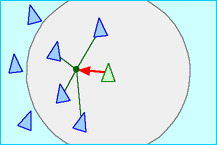
\includegraphics[scale=0.5]{co-0000}
            \caption{Cohesion Rule\cite{boids}}
        \end{figure}
        The cohesion rule ensures agents stick together.
    }
    \only<1->{
    
    The cohesion move vector $\vec{C}$ can be represented as follows:
    
    \[
    \vec{C} = \begin{cases}
    0 & \text{if } |N| = 0 \\
    \frac{1}{n_{avoid}}\sum_{n=1}^{|N|} \vec{a} - \vec{n} & \text{otherwise}
    \end{cases}
    \]
    
    }
    
\end{frame}

\subsection{Pathfinding}
\begin{frame}
    \frametitle{Boids!}
    \only<1->{
        So we have our three fundamental behaviours.
    }
    \\
    \only<1->{
        \begin{figure}
            \centering
            \animategraphics[autoplay,loop,controls,width=0.8\linewidth]{10}{boids-}{0}{279}
            \caption{Emergent Behaviour\cite{rafaelkuebler_2018}}
        \end{figure}
    }
\end{frame}

\begin{frame}
    \frametitle{Seeking}
    \onslide<1->{
        We now look to add the ability to seek a given goal to our agents.
        \\
        We will assume the location of the goal is known.
        \begin{columns}
            \column{0.5\textwidth}
            \centering
                \begin{figure}
                    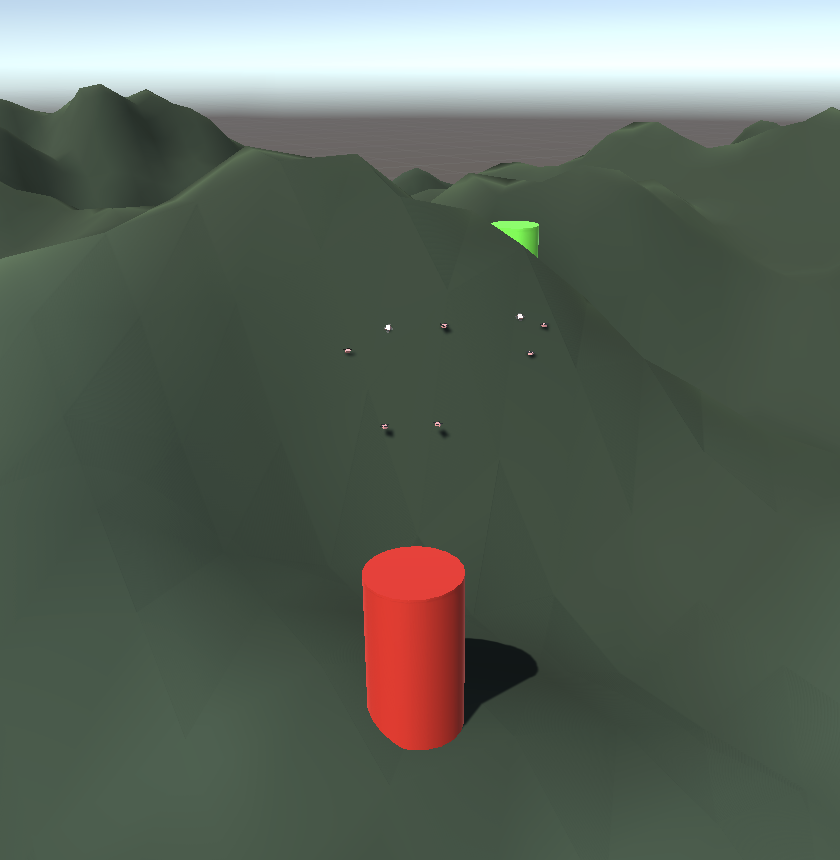
\includegraphics[width=0.5\linewidth]{startplatform}
                    \caption{Start Platform}
                \end{figure}
            \column{0.5\textwidth}
            \centering
                \begin{figure}
                    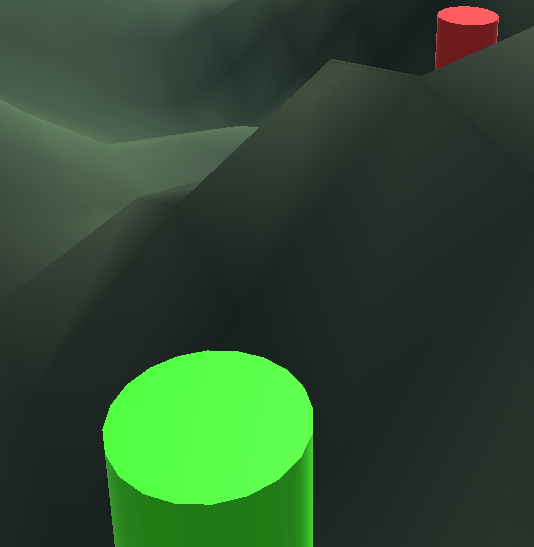
\includegraphics[width=0.5\linewidth]{goalplatform}
                    \caption{Goal Platform}
                \end{figure}
            
        \end{columns}
    }
    \onslide<1->{
        This can be done by calculating the vector between the goal position and the current position of the agent.
        $$
        \vec{D} = \vec{goal} - \vec{agent}
        $$
    }
\end{frame}

\subsection{Terrain}

\begin{frame}
    \frametitle{Terrain Generation}
    \onslide<1->{Terrain was generated using \emph{Perlin Noise}, introduced by Ken Perlin in 1983.}
    \\
    \onslide<1->{

        \begin{figure}
            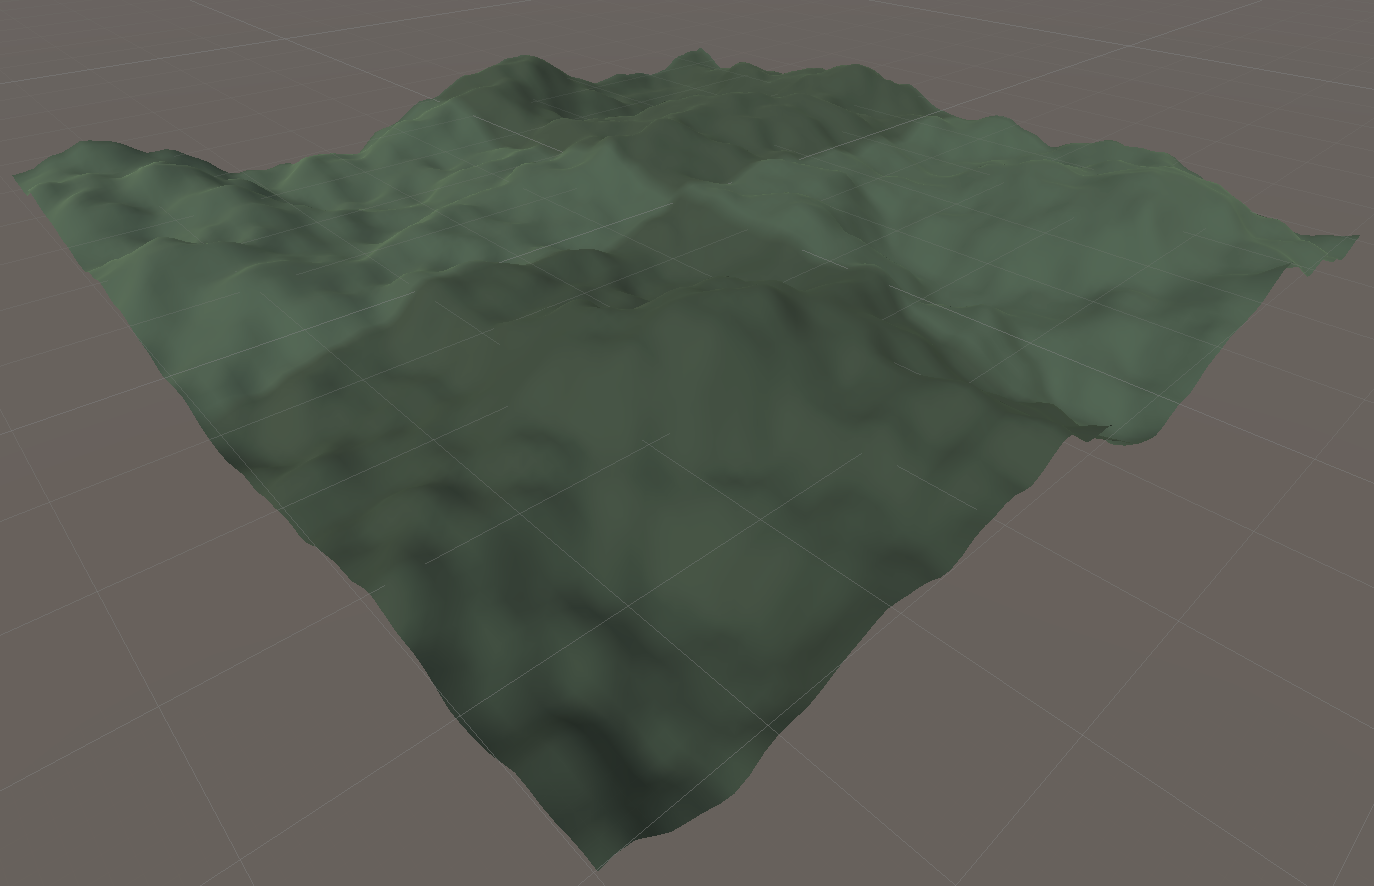
\includegraphics[scale=0.2]{lacunarity2}
            \caption{Perlin Noise Terrain}
        \end{figure}
    }
\end{frame}

\begin{frame}
    \frametitle{Terrain Avoidance}
    \onslide<1->{To implement the avoidance behaviour, we can simulate a \emph{ranging} sensor ray on the agents.}
    \\
    \onslide<1->{
        We can then apply an upward thrust when the distance to the terrain is below a certain threshold.
        $$
            vec(E) = \begin{cases}
                0 & \text{if } d > R_{avoid} \\
                (0,c_{thrust},0) & \text{otherwise}
            \end{cases}
        $$
    }
    \onslide<1->{
        \begin{figure}
            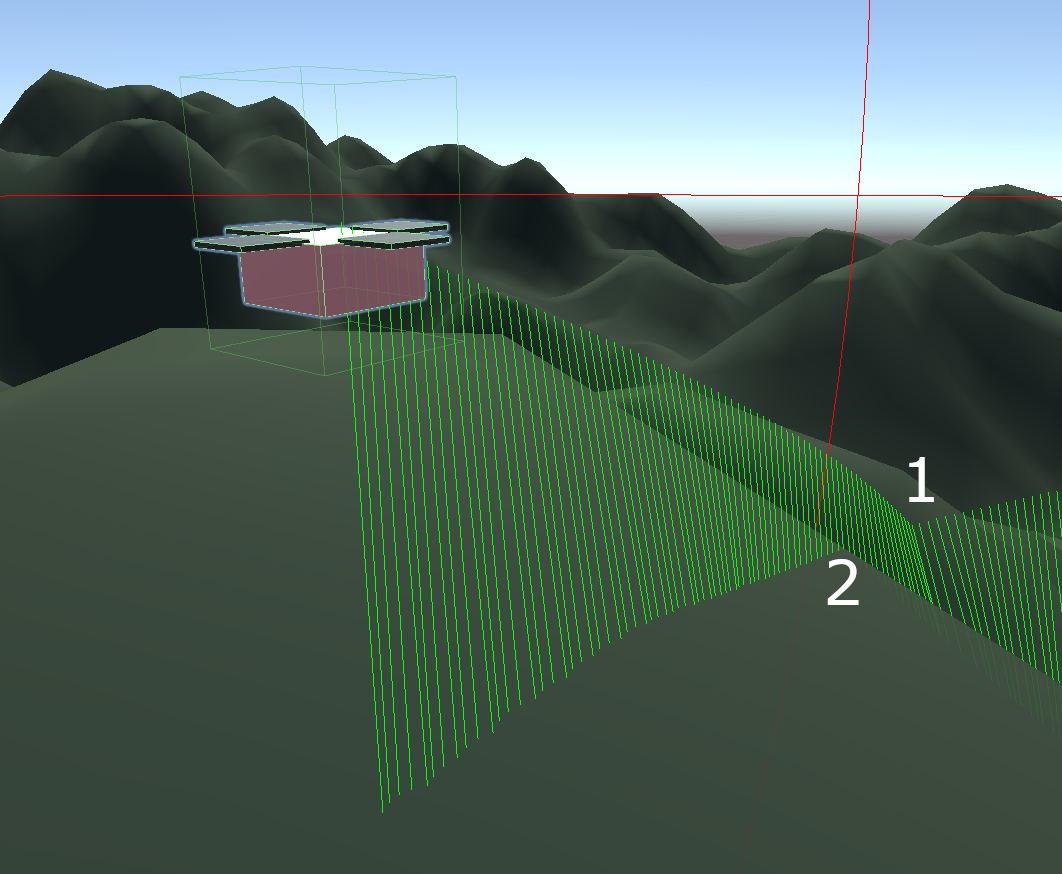
\includegraphics[scale=0.2]{naive-ta-edited}
            \caption{Agent with incident rays}
        \end{figure}
    }

\end{frame}

\subsection{Parameter Optimisation}
\begin{frame}
    \frametitle{Composite Behaviour}
    \onslide<1->{
        \begin{block}{Optimisation}
            We can use a bounded linear combination of the rules to control the behaviour of our UAVs.
        \end{block}
    }
    \onslide<1->{
        $$
        \vec{New} = \alpha \vec{A} + \beta \vec{B} + \gamma \vec{C} + \delta \vec{D} + \epsilon \vec{E}
        $$
    }
    \\
    \onslide<1->{
        \alert<1->{Problem: How can we calculate the best values for $\alpha, \beta, \gamma, \delta, \epsilon$?}
    }

\end{frame}

\begin{frame}
    \frametitle{Simulated Annealing}
    We can define three `scenarios' and a cost function to optimise the behaviour of the drones. We can then use a simulated annealing algorithm to find the best parameter values.

    The scenarios chosen were:
    \begin{itemize}
        \item Shortest First-Arrival Time
        \item Reduced Spread (Cohesivity)
        \item Reduced Collisions
    \end{itemize}

    A modular cost function was defined to calculate the cost of the parameters in each scenario.

\end{frame}

\section{Interim Results}

\begin{frame}
    \frametitle{Optimisation: Shortest First-Arrival Time}
    \onslide<1->{We can see the effect of the parameters on the first-arrival time by the optimised parameter values:}
    \onslide<1->{
        \begin{table}
            \begin{tabular}{|c|c|}
                \hline
                Parameter & Value \\
                \hline
                Avoidance & 8.5 \\
                Alignment & 2.5 \\
                Cohesion & 0.5 \\
                Seeking & 17 \\
                Terrain Avoidance & 16.5 \\
                \hline
            \end{tabular}
            \caption{Optimised Parameters for Shortest First-Arrival Time, $c = 0.268$}
        \end{table}
    }
\end{frame}

\begin{frame}
    \frametitle{Optimisation: Reduced Spread}
    \onslide<1->{We can consider the case where we want to reduce the spread of the agents' arrival time at the goal. We have found the optimised parameter values:}
    \onslide<1->{
        \begin{table}
            \begin{tabular}{|c|c|}
                \hline
                Parameter & Value \\
                \hline
                Avoidance & 12.5 \\
                Alignment & 4 \\
                Cohesion & 15 \\
                Seeking & 18.5 \\
                Terrain Avoidance & 0.5 \\
                \hline
            \end{tabular}
            \caption{Optimised Parameters for Reduced Spread, $c = 0.229$}
        \end{table}
    }

\end{frame}

\begin{frame}
    \frametitle{Optimisation: Reduced Spread}
    We can also explore the trajectory of the simulations to see how the annealing schedule affects the paramters of the cost function.
    \begin{figure}
        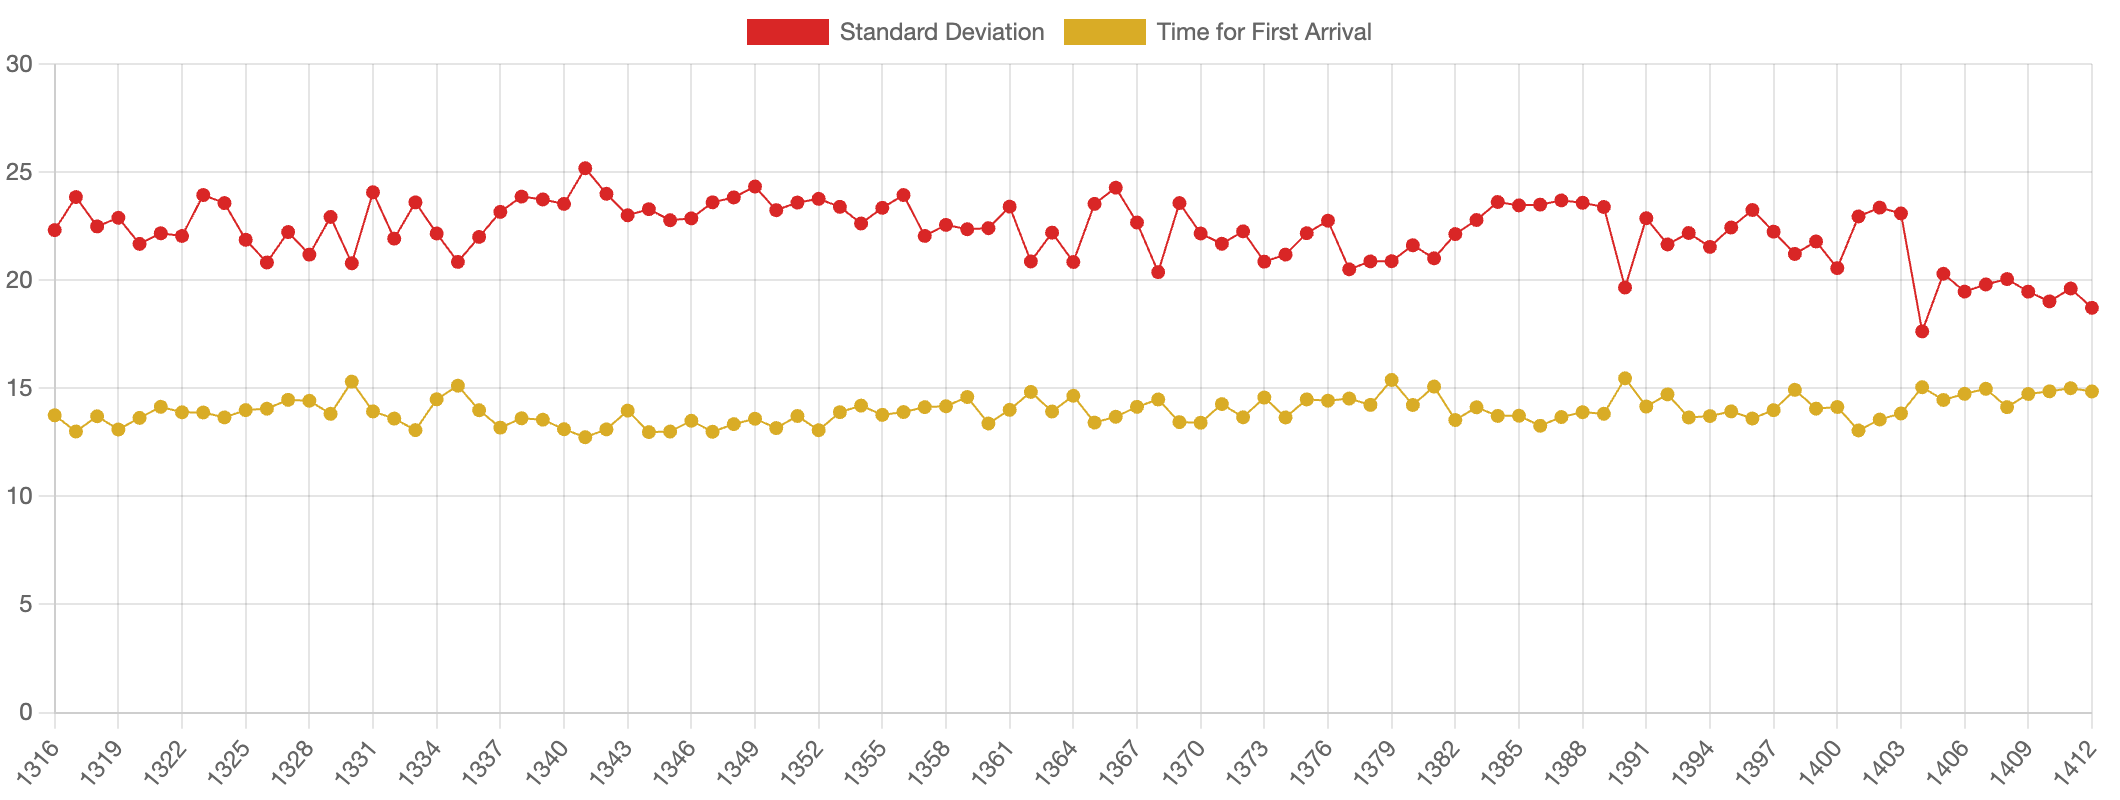
\includegraphics[width=0.7\linewidth]{chart}
        \caption{One SA Simulation Run}
    \end{figure}
    

    Issue 1: The chosen parameters may not have the intended effect on chosen observations.

\end{frame}

\begin{frame}
    \frametitle{Optimisation: Reduced Collisions}
    Looking at minimising collisions, we notice that the effect of the parameters on the cost function is not always as would be expected.
    \begin{enumerate}
        \item Collision numbers are not bounded.
        \item Random spawn points mean a large range of initial conditions.
    \end{enumerate}
    For example, for one of the lowest cost functions:
    \begin{table}
        \begin{tabular}{|c|c|}
            \hline
            Parameter & Value \\
            \hline
            Avoidance & 3 \\
            Alignment & 15 \\
            Cohesion & 15.5 \\
            Seeking & 4.5 \\
            Terrain Avoidance & 2.5 \\
            \hline
        \end{tabular}
        \caption{Optimised Parameters for Reduced Collisions, $c = 0.202$}
    \end{table}
    Issue 2: Simulated Annealing does not always find the global minimum.
\end{frame}



\section{Project Management}
\begin{frame}
    \frametitle{Status Update}
    \begin{figure}
        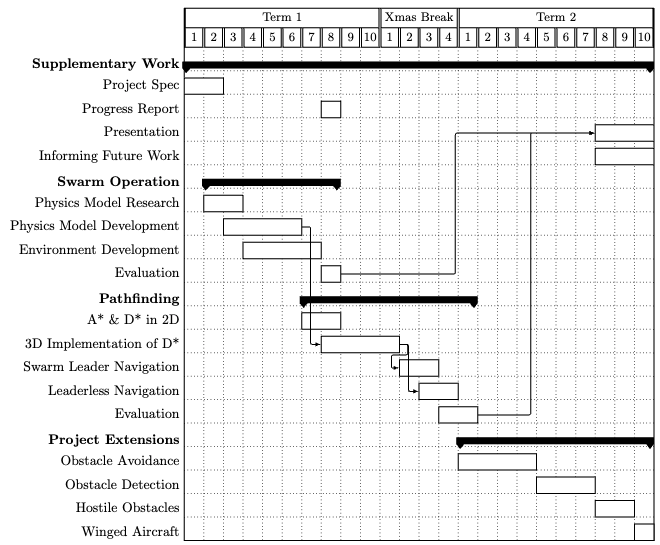
\includegraphics[width=0.6\linewidth]{gantt}
        \caption{Gantt Chart}
    \end{figure}
\end{frame}

\section{Future Work}

\begin{frame}
    \frametitle{Future Work: Solving the Issues?}
    \onslide<1->{
        \begin{block}{Issues}
            \begin{enumerate}
                \item Chosen parameters may not have the intended effect on chosen observations. Curse of dimensionality?!
                \item Simulated Annealing does not always find the global minimum.
            \end{enumerate}
        \end{block}
    }
    \onslide<2->{
        To solve this, we will aim to look at alternative optimisation algorithms and tweak our behaviours.
        \begin{itemize}
            \item Boids (1987) vs Boids (1999)?
            \item Particle Swarm Optimisation?
        \end{itemize}
        The focus has been on controlling specific behaviours, which contribute to a goal state. What if we control the goal state itself?
    }
\end{frame}

\begin{frame}
    \frametitle{Future Work: Extensions}
    We have successfully implemented the pathfinding and control of a basic swarm of UAVs.
    \\
    The hope is that we can introduce other kinds of obstacles into the simulation, much like terrain currently.
    \\
    \bigskip
    An interesting extension involves the introduction of hostile agents into the simulation, with the ability to avoid these agents or even `fight back' in some cases.
\end{frame}

\section{Conclusion}
\begin{frame}
    \centering
    
\includegraphics[width=0.1\linewidth]{logo}
    \bibliographystyle{plain}
    \bibliography{refs}
\end{frame}

\end{document}